\scanpage{24}
\mspage{\textcircled{6}}

\textsf{\textbf{ACADEMY OF AIX-MARSEILLE}}\\
\rule{3cm}{.4pt}\\
\textbf{ACADEMIC INSPECTORATE}\\
\textbf{OF VAUCLUSE}\\
\rule{1cm}{.4pt}

What is the subset of $X_2\times X_2$ that comes from $X'_3$ ?

\[
\text{a)}\quad(p,p\rho)(e_3)=(e_2,e_2)
\]
\[
\text{b)}\quad(p,p\rho)
\underset{\substack{i\in\mathbb Z/3\mathbb Z\\\unsure{\xi|\zeta}\in X_2^*=X_2\setminus\{e_2\}}}{
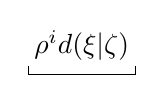
\begin{tikzpicture}[baseline=(term.base)]
\node[inner sep=1pt] (term) {$\rho^i d(\unsure{\xi|\zeta})$};
\draw[line width=.45pt] ([xshift=-1pt,yshift=-1pt]term.south west) -- ([xshift=-1pt,yshift=-4pt]term.south west) -- ([xshift=1pt,yshift=-4pt]term.south east) -- ([xshift=1pt,yshift=-1pt]term.south east);
\end{tikzpicture}}
=\begin{cases}
(\unsure{\xi|\zeta},e_2)&\text{if }i=0\\
(e_2,\sigma\unsure{\xi|\zeta})&\text{if }i=1\\
(\sigma\unsure{\xi|\zeta},\unsure{\xi|\zeta})&\text{if }i=2
\end{cases}
\]

So we find the elements \deleted{of the \unsure{form}} in
\[
\uline{\underbrace{(X_2\times\{e_2\})}_{\Sigma_1}\cup\underbrace{(\{e_2\}\times X_2)}_{\Sigma_2}\cup\deleted{\unsure{\Delta}}\Delta'}
\]
where $\Delta'$ is the image of
\figure{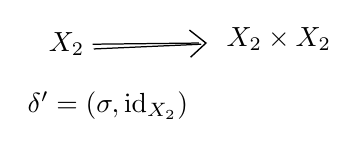
\begin{tikzpicture}[x=.015cm,y=.015cm,every node/.style={inner sep=0pt}]
\node[anchor=base] at (0,0) {$X_2$};
\node[anchor=base west] at (135,4) {$X_2\times X_2$};
\node[anchor=base] at (35,-52) {$\delta'=(\sigma,\mathrm{id}_{X_2})$};
\draw[line width=.45pt] (22,6) -- (112,7);
\draw[line width=.45pt] (23,2) -- (114,6);
\draw[line width=.5pt] (104,18) -- (118,7) -- (105,-5);
\end{tikzpicture}}

\uline{NB} This subset $\Sigma$ of $X_2\times X_2$ is the union of $\Sigma_{\unsure{1|0}},\Sigma_2,\Delta'$, the intersection of any two of the three being equal to $\{(e_2,e_2)\}$

When do we have $\Sigma=X_2\times X_2$ ?

\deleted{\unsure{If}} We have
\[
X_2\times X_2\longrightarrow\{\Sigma_1\cup\Sigma_2)=X_2^*\times X_2^*,
\]
so it is necessary and sufficient that $X_2^*\longrightarrow X_2^*\times X_2^*$ be surjective, i.e. that for $\unsure{\zeta|\xi},\eta\in X_2^*$, we always have $\eta=\sigma\unsure{\zeta|\xi}$. This means that we are in one of the following 2 cases

a) $X_2^*=\unsure{\phi|\varnothing}$ i.e. $X_2=\{e_2\}$

b) $X_2^*$ of cardinality 1 (so $\sigma$ \deleted{\unsure{on it}} acts on it \unsure{trivially})

\reversemarginpar
\margin{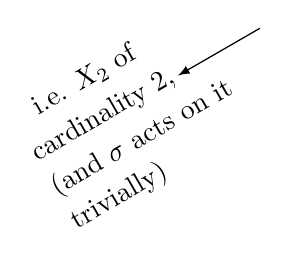
\begin{tikzpicture}[rotate=30,transform shape,every node/.style={inner sep=0pt}]
\node[anchor=base west] at (0,0) {i.e. $X_2$ of};
\node[anchor=base west] at (-.3,-.5) {cardinality $2$,};
\node[anchor=base west] at (-.3,-1) {(and $\sigma$ acts on it};
\node[anchor=base west] at (-.3,-1.5) {\unsure{trivially})};
\draw[-latex,line width=.45pt] (3,-.45) -- (1.8,-.45);
\end{tikzpicture}}
\normalmarginpar

[If $X_2^*$ has cardinality $\geq2$, then if there is a single orbit under $\sigma$, it has cardinality 2, and \deleted{$\unsure{\xi}$} $\forall\unsure{\zeta|\xi}\in X_2^*)$ $(\unsure{\zeta|\xi},\unsure{\zeta|\xi})\notin\operatorname{Im}\delta'$ i.e. $\unsure{\zeta|\xi}\ne\sigma\unsure{\zeta|\xi}$). or if there are \deleted{\unsure{two|so}} at least two orbits, we take $\unsure{\zeta|\xi},\eta$ in two different orbits, and we indeed have $\eta\ne\sigma\unsure{\zeta|\xi}$.

\margin{23}
